\documentclass[12pt,a4paper]{scrartcl}
\usepackage[utf8]{inputenc}		% ermöglich die direkte Eingabe der Umlaute 
\usepackage[T1]{fontenc}		% das Trennen der Umlaute
\usepackage[ngerman]{babel}		% hiermit werden deutsche Bezeichnungen genutzt 
\usepackage{csquotes} 			% Gänsefüßchen nach gesetzter Sprache
\usepackage{graphicx}			% Bilder
\usepackage{subcaption}			% Für die Subfigures
\usepackage{geometry}			% Seitengröße
\usepackage[backend=biber,style=numeric,]{biblatex}	% Für das Literatursverzeichis
\usepackage{glossaries}			% Für Glossar
\usepackage{caption}			% Für schicke Titel bei Figures und Tabellen
\usepackage{chngcntr}			% Zähler für Figures und Tabellen anpassen
\usepackage{titling}			% Für schicke Titel
\usepackage{helvet}				% Für Helvetica 
\usepackage[onehalfspacing]{setspace}	% Seitenabstände
\usepackage{fancyhdr}			% Für die Kopf- und Fußzeile
\makeglossaries					% Glossar 
\counterwithin{figure}{section}	% Zähler
\counterwithin{table}{section}
\renewcommand{\familydefault}{\sfdefault}	% Auch wegen Font
\geometry{						% Seitengröße
  left=2.5cm,
  right=2.5cm,
  top=2.5cm,
  bottom=2cm,
  bindingoffset=5mm
}
\pagestyle{fancy}				% Stil setzen
\lhead{Containervirtualisierung und horizontale Skalierung}	% Header
\rhead{}\chead{}				% Andere Header leeren
\rfoot{Seite \thepage}
\lfoot{}\cfoot{}
\loadglsentries{glossary.bib}	% Datenfiles einfügen
\addbibresource{literatur.bib}

%------------------------
% Deckblatt Titel und co.
%------------------------

\pretitle{\begin{center}
\begin{figure}[h!]
	\begin{subfigure}{0.2\linewidth}
		
\includegraphics[scale=1]{DHBWLogo.png} 
	\end{subfigure}
	\hspace*{\fill}
	\begin{subfigure}{0.3\linewidth}
    	
\includegraphics[scale=0.25]{YellowMap.png}
	\end{subfigure}
\end{figure}
}
\posttitle{\end{center}}
\title{\Large{\bfseries Containervirtualisierung und horizontale Skalierung}\vspace{1cm}
	\large PRAXISBERICHT\vspace{1cm}}
\author{
	\normalsize für die Prüfung zum\\
	\normalsize Bachelor of Engineering/Bachelor of Science\\
	\normalsize des Studiengangs Informatik\\
	\normalsize Studienrichtung Angewandte Informatik\\
	\normalsize an der\\
	\normalsize Dualen Hochschule Baden-Württemberg Karlsruhe\\\\
	\normalsize von\\
	\normalsize Jakob Jonathan Heitzmann
}
\date{\today}
\begin{document}

\maketitle
\vspace*{\fill}
\thispagestyle{empty}

%----------------
% Deckblatt unten
%----------------


\begin{tabular}{p{5cm}ll}
	Matrikelnummer & 9119328\\
	Kurs & TINF19B4\\
	Ausbildungsfirma & YellowMap AG, & Karlsruhe\\
	Betreuer & Markus Lind\\
	Prof. Jörn Eisenbiegler
\end{tabular}

\newpage

%--------------------------
% Eidesstattliche Erklärung
%--------------------------

\section*{Erkl\"arung}

Gem\"a\ss\ \S\ 5 (3) der ''Studien- und Pr\"ufungsordnung DHBW Technik'' vom 29. September 2017 erkl\"are ich, Jakob Jonathan Heitzmann, dass ich die vorliegende Arbeit selbstst\"andig verfasst und keine anderen als die angegebenen Quellen und Hilfsmittel verwendet habe, sowie dass die physisch-vorliegende Version der Digitalen identisch ist.\\

\hspace*{0.5cm}
Karlsruhe, den \today

\vspace*{2cm}

\begin{tabular}{@{}l@{}}\hline
\rule{0pt}{2ex}
Jakob Jonathan Heitzmann
\end{tabular}
\newpage

\tableofcontents
\addcontentsline{toc}{section}{Inhaltsverzeichnis}
\newpage
\listoffigures
\addcontentsline{toc}{section}{Abbildungsverzeichnis}
\newpage
\listoftables
\addcontentsline{toc}{section}{Tabellenverzeichnis}
\newpage
\printglossary
\addcontentsline{toc}{section}{Glossar}
\newpage

%-----------------------------------------------------------------------------------------------
%Hier beginnt das eigentliche Inhalt des Dokuments. (Davor nur Deckblatt bis Inhaltsverzeichniss)
%-----------------------------------------------------------------------------------------------

\section{Einf\"uhrung}
Ziel der Arbeit ist es vorzuzeigen was ich in den ersten beiden Semestern meines Studiums bei der YellowMap AG gelernt und getan habe. Dabei wird sich auf die Gesamtheit der Bemühungen begrenzt, die dazu galten die bestehende Serverstruktur zu brechen und einen Prototypen zu konzeptionieren, mit wessen Vorbild man das bestehende System in ein verteiltes System wandeln könnte. Zu diesem Zweck musste ich mich mit verschiedenen Arten der Serverkommunikation und Containervirtualisierung beschäftigen.

\subsection{Kontextuelle Betrachtung der Rahmenbedingungen}

YellowMap entwickelt und hostet in erster Linie Kartenanwendungen, bietet Entwicklern aber auch mit einer Java-Script-API die Möglichkeit mit wenig Selbstaufwand selbst eine solche Anwendung zu Entwickeln. Dabei laufen die Dienste mit allen gängigen großen Kartenanbietern so wie Google, OSM, Bing und sogar Baidu. Exemplarische Lösungen, die YellowMap anbietet, sind zum Beispiel die FilialFinder, mit denen alle Filialen eines Klienten auf dessen Webseite angezeigt werden können. Die Anzeige erfolgt natürlich auf einer Karte. Gesucht wird für gewöhnlich mit einer Umkreissuche auf den Standort des Gerätes. Die Gefundenen Filialen können auch neben der Karte auch auf einer Liste sortiert ausgegeben werden.

\begin{figure}[h!]
	\centering
	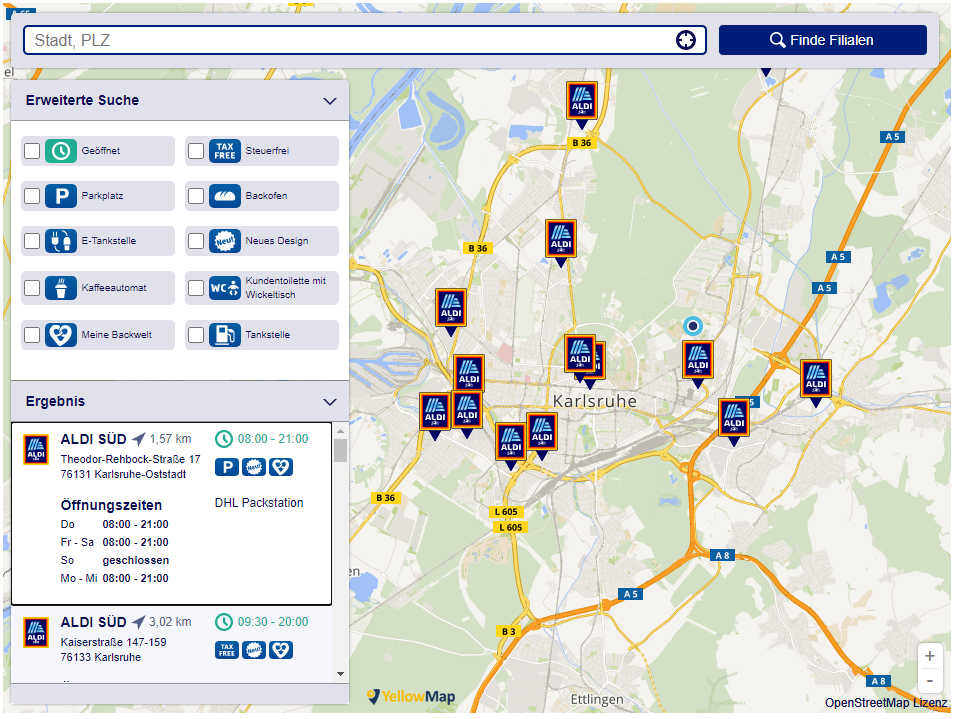
\includegraphics[scale=0.55]{YmFF.png}
	\caption[https://www.aldi-sued.de/filialen/]{FilialFinder}
\end{figure}

%Redo
%Zu Beginn bekam ich diverse Sonderaufgaben zugeteilt, die zu meiner Einarbeitung dienten. 
Im umrissenen Zeitraum habe ich viele Tätigkeiten besonders in den Bereichen Backend und Testing übernommen. Doch auch ein paar kleinere Aufgaben im Bereich Frontend fielen mir zu. Gearbeitet habe ich mit .NET Core, Gatling, HTML, CSS, JavaScript, Docker, Kubernetes und RabbitMQ. 
Darunter war die Entwicklung eines Dienstes, der dazu fähig ist Termindaten von einer Datenbank zu ziehen und diese dann auf kleinen E-Paper-Bildschirmen anzuzeigen was vollständig in C\# realisiert wurde. Auch entwickelte ich zu Demozwecken Testwebseiten die Funktionen der JavaScript API präsentieren sollten. Ein anderes Projekt war die Realisierung von Stresstests auf ein schon bestehendes Projekt mittels Gatling. Dafür musste ich mich in die Programmiersprache Scala und Maven einarbeiten. 

Das Projekt, auf das ich in diesem Bericht näher eingehen möchte war nun die Entwicklung eines Prototyps zur Containervirtualisierung und automatischen horizontalen Skalierung mittels Docker und Kubernetes, sowie die Entwicklung eines Prototyps für die Serverkommunikation mit Message Broker mittels RabbitMQ. Für diese Aufgabe wurden diese Technologien vorgegeben. 

\subsection{Das bisherige Serverdesign}
Das bestehende System wurde entworfen damit viele Anwendungen unabhängig voneinander entwickelt werden können ohne, dass jede Funktionalität in jeder neuen Anwendung auch neu geschrieben werden müsste. Dazu greifen alle Projekte auf dieselbe Schnittstelle zu, diese bietet dann die einzelnen Funktionalitäten in einem einheitlichen Format. Diese Art der Kommunikation ermöglicht es unabhängig von Art der Anwendung die Anbindung an die internen Dienste sicherzustellen. Eine Anfrage eines Projekts auf diese Schnittstelle landet als erstes am Proxy der Core, also zu Deutsch dem Kern, hier wird die Anfrage angenommen und auf erster Ebene Authentifiziert. Diese Anfrage wird dann an den System Call weitergeleitet. Hier befindet sich der Partnerschalter. Er reichert die Daten der Anfrage mit den Daten zum gelieferten Partner aus der Datenbank an. Heißt er schaut zum Beispiel von welchem Provider der Partner seine Daten beziehen möchte und trifft dem entsprechend Vorkehrungen, dass die Daten in den folgenden Aufrufen und Aktionen richtig weitergegeben und verarbeitet werden. Auch wird hier die auszuführende Aktion ermittelt und der dazugehörige Befehl in Form eines Commands oder einer Command-Group. Ein Command reichert die Daten nun weiter an und reicht dann an einen Provider spezifische Command-Action weiter, die die angefragte Aktion dann ausführt. In Abbildung 7.1 sehen wir so einen Aufruf, der dann aber Beispielshalber auf ein Lagacy-System zugreift, das wiederum selbst eine eigene Command-Action besitzt, die die Anfrage dann letztendlich ausführt. Diese Legacy-Systeme werden aber in dieser Arbeit nicht weiter betrachtet, da diese nicht mehr aktiv weiterentwickelt werden.

\begin{figure}[h!]
	\centering
	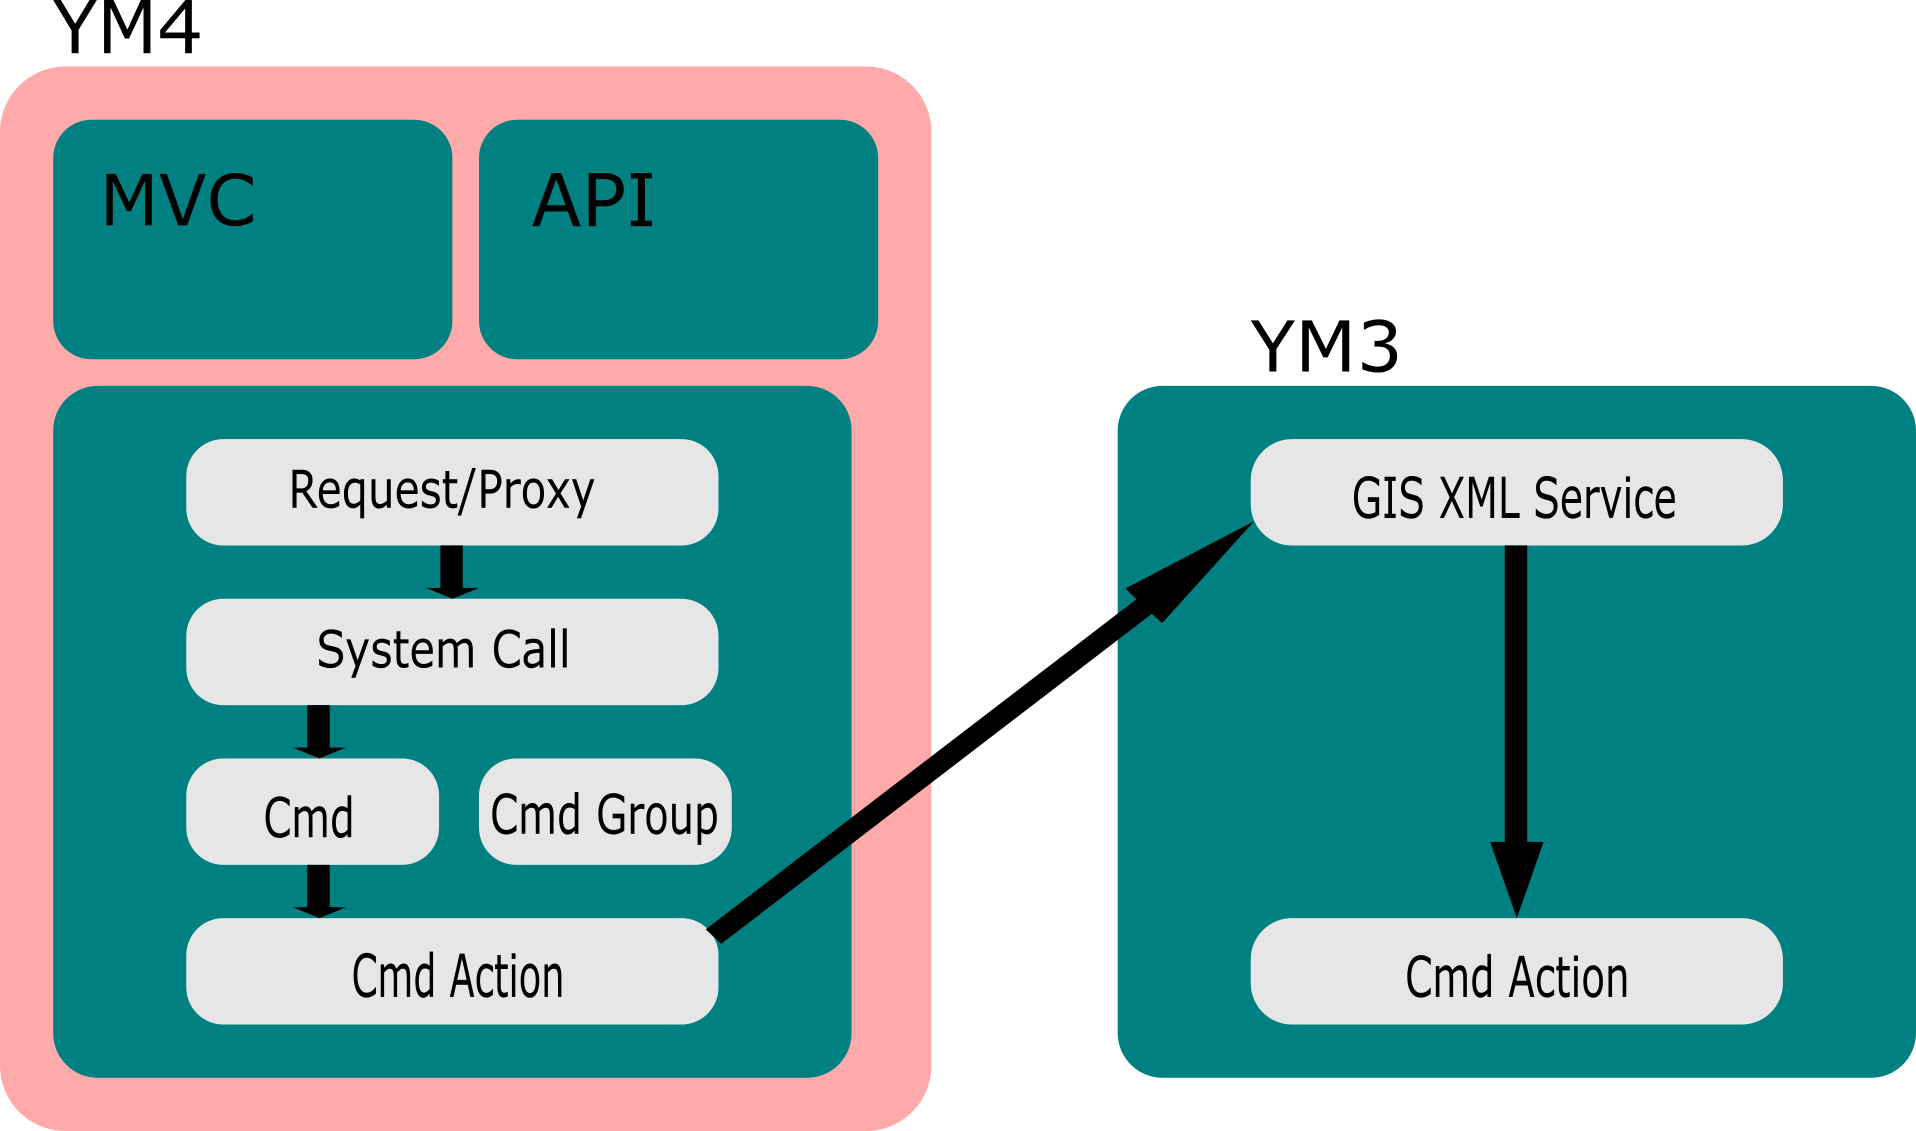
\includegraphics[scale=2]{YmSysReq.png}
	\caption[Selbst erstellte Grafik]{Beispielanfrage}
\end{figure}

Das System ist also kein Monolithisches, da es aus vielen Einzelprojekten besteht, die größtenteils unabhängig von einander agieren können, aber es ist ebenso kein verteiltes System, da sich trotz des modularen Designs alles auf demselben Server befindet.

\section{Serverkommunikation mit Message Broker} \label{rabbit}
Zuerst begann ich den Prototypen für die Serverkommunikation mittels Message Broker zu konzeptionieren. Der Message Broker sollte eine neue interne Schnittstelle zwischen dem Serversystem und dem Legacy-System etablieren, da diese zuvor via normale HTTP-Aufrufe, die über das externe Netz gingen, realisiert wurde. Dies benötigte das Herauslösen eigenständiger Komponenten des Legacy-Systems und die Umwandlung dieser in sogenannte Microservices. Im Hinblick auf die späteren Änderungen, die noch an dem System vorgenommen werden sollten, sollte auch die Möglichkeit betrachtet werden, die Protokollierung von Systemdaten über den Message Broker auf eine Vielzahl von Empfängersystemen zu ermöglichen. 

\subsection{Funktion eines Message Brokers}
Ein Message Broker ist ein System zur Nachrichtenübertragung und Nachrichtenverteilung. Dafür fungiert der Message Broker selbst als der zentrale Umschlagplatz von dem aus Nachrichten Empfangen und Verteilt werden. Ebenso übersetzt er aktiv zwischen verschiedenen Protokollen\cite{mesBro}. Er stellt eine Art Middleware da, was bedeutet, dass er als neutrale Komponente im System nur für die Vermittlung von Information zwischen anderen Komponenten verantwortlich ist.

\subsection{Anwendungsspezifische Betrachtung}
In Hinblick auf die Containervirtualisierung ist das Prinzip eines Message Brokers mehr als nützlich.
Ein Message Broker kann einen Nachrichten-Pool schaffen, den er kontinuierlich und gezielt mit Nachrichten versorgt, die dann von den letztendlichen Verbrauchern konsumiert werden können. Dadurch schafft man ein Netz von Geräten, die nur noch eine zentrale Adresse kennen müssen und dadurch dynamischer und unabhängiger voneinander agieren können. 

\begin{figure}[h!]
	\centering
	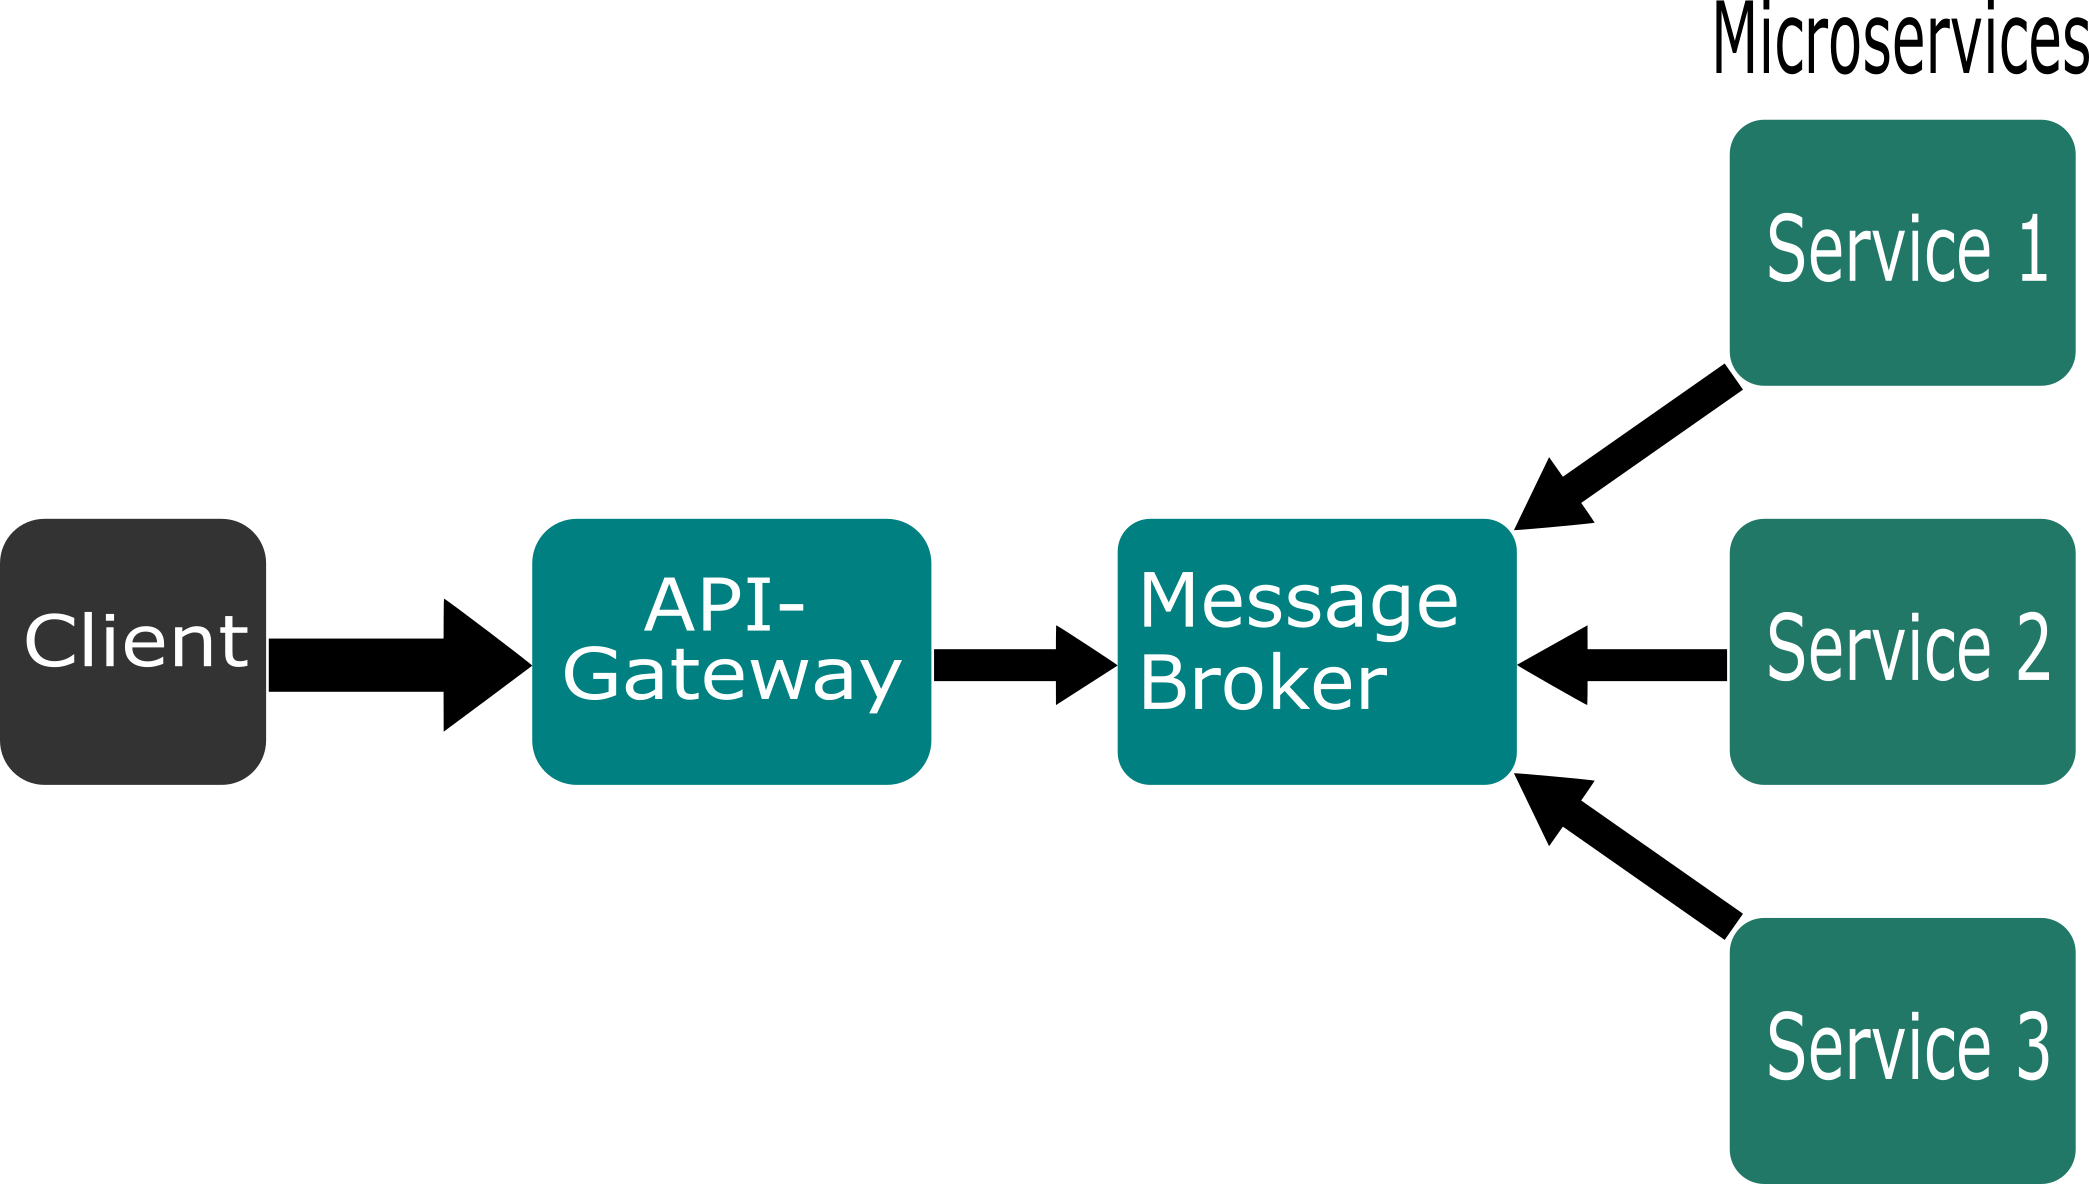
\includegraphics[scale=1.8]{MesBroSys.png}
	\caption[Selbst erstellte Grafik]{Serversystem mit Message Broker}
\end{figure}

In Abbildung 8.1 sehen wir wie der Message Broker seine Funktion als Middleware zwischen einem API-Gateway und mehreren Diensten erfüllt.  

\subsection{RabbitMQ}
RabbitMQ ist ein Open-Source-Message-Broker, der das Advanced-Message-Queuing-Protokoll (AMQP) unterstützt und sogar um einige nützliche Funktionalitäten erweitert\cite{rabExt}.
Darunter ist eine grafische Managementoberfläche und Unterstützung für Remote-Procedure-Calls (RPC). Dies sind beides Funktionen die enormst praktisch für die vorgesehene Verwendung sind.

Mittels grafischer Managementoberfläche wird die Fehlersuche immens einfacher Gestaltet. Sie zeigt an, an welchen Endpunkten Nachrichten eingetroffen sind, wie viele es sind, ob ein Endpunkt gemeldete Konsumenten hat und vieles mehr. Mit ihr kann man ebenfalls sämtliche Konstrukte selbst erzeugen und die Nachrichten im allgemeinen Verwalten. 

Ein RPC ermöglicht es uns eine Funktion auf einem anderen Gerät auszuführen und ebenso dessen Wert zurückgeliefert zu bekommen. Was genau das ist was wir in einem verteilten System wollen.

\subsubsection{Grundlegende Funktionsweise}

RabbitMQ stellt in erster Linie einen Serverdienst, eine Managementoberfläche und Nutzerschnittstellen zur Verfügung. Der Serverdienst nimmt Nachrichten entgegen und Verwaltet diese. 
Er besitzt Exchanges und Queues. Ein Exchange nimmt eine Nachricht entgegen und verteilt diese an eine oder mehrere Queues, die ein Binding auf den jeweiligen Exchange haben. 

\begin{figure}[h!]
	\centering
	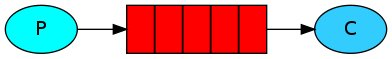
\includegraphics[scale=1]{P2C.jpg}
	\caption[https://www.rabbitmq.com/tutorials/tutorial-one-dotnet.html]{Produzent, Queue und Konsument}
\end{figure}

Es gibt verschiedene Arten von Exchanges, die Nachrichten auf verschiedene Weise verteilen. 

Ein Fanout-Exchange sendet die Nachricht an jede Queue, mit der er ein Binding besitzt. 

Ein Direct-Exchange sendet eine Nachricht nur an eine Queue, wenn der Routing-Key der Nachricht mit dem Namen einer Queue übereinstimmt, die natürlich auch ein Binding auf dem Exchange haben muss.

\begin{figure}[h!]
	\centering
	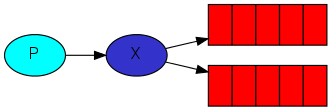
\includegraphics[scale=1.65]{exchanges.png}
	\caption[https://www.rabbitmq.com/tutorials/tutorial-three-dotnet.html]{Produzent, Exchange und Queue}
\end{figure}

Ein Topic-Exchange wiederum verteilt an mehrere Queues in seinem Binding. Dabei dürfen die Queues keinen willkürlichen Namen tragen, sondern müssen einem gewissen Namensmuster Folgen, dass teilweise den Routing-Key der zu empfangenden Nachrichten reflektieren soll. Wenn zum Beispiel der Routing-Key einer Nachricht core.failure.critical wäre, so wäre auch *.*.critical ein Name, unter dem eine Queue diese Nachricht empfangen würde. Dabei steht das Sternchen als Platzhalter für jedes mögliche Wort. Die Punkte reflektieren die Punkte im Routing-Key. Eine Raute ist dabei ein Platzhalter für mehrere Wörter, also über Punkte hinaus. 

Der Standard-Exchange ist ein Direct-Exchange und wird innerhalb des Codes mit Hilfe einer Leeren Zeichenkette ausgewählt. Er ist auch notwendigerweise mit allen Queues verbunden.

Ein Exchange wird von Produzenten befüllt. Ein Produzent erzeugt Nachrichten und schickt diese an Exchanges damit diese dann an einer oder mehreren Queues konsumiert werden.

Eine Queue ist ein Speicher, der Nachrichten zwischenspeichert und nach dem First-in-First-Out (FIFO)-Prinzip an Konsumenten verteilt. Sie sind Anlaufstelle für Konsumenten. 

Ein Konsument meldet sich bei einer Queue und wird dort in eine Liste von Konsumenten aufgenommen. So wird er dann von dem Server mit Nachrichten bedient. Wird eine Nachricht konsumiert kann ein Konsument diesen Vorgang bestätigen falls der Produzent es wünscht. Das heißt wiederum aber auch, dass der Produzent nun auch auf die Antwort des Konsumenten wartet und ihn somit potenziell Blockiert.

Eine Nachricht wird in RabbitMQ mit vielen Attributen abgesendet. Sie folgt in erster Linie dem AMQP, doch RabbitMQ hat diese um einige Funktionen erweitert. So kommt zum Beispiel das Attribut reply\_to mit. In diesem Attribut kann eine Antwortadresse für zum Beispiel den Absender hinzugefügt werden. Dieses Attribut wird später im Remote-Procedure-Call benutzt. Sonst kommt offensichtlicherweise Informationen über die Zieladresse und den Ziel-Exchange, der Routing-Key und natürlich auch die eigentliche Nachricht, dem Body, mit.

Die Managementoberfläche und Nutzerschnittstellen bieten eine Plattform, von der man mit dem Serverdienst wie beschrieben interagieren kann.

\subsubsection{Remote-Procedure-Call (RPC)}
Der RPC ist ein Muster, das uns ermöglicht auf eine Nachricht eine entsprechende Antwort zu bekommen, wie bei einem Funktionsaufruf. 

\begin{figure}[h!]
	\centering
	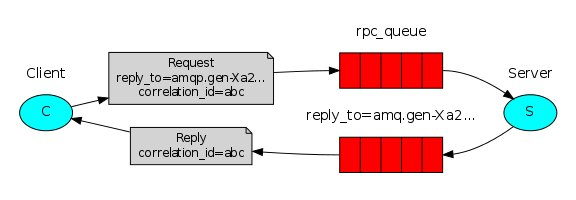
\includegraphics[scale=0.74]{RPC.jpg}
	\caption[https://www.rabbitmq.com/tutorials/tutorial-six-dotnet.html]{RPC}
\end{figure}

Für dieses Muster verwenden wir zuerst einen normalen Produzenten, den wir jedoch um die Attribute reply\_to und correlation\_id erweitern. Wir setzten die Antwort-Queue auf einen zufälligen Namen, den wir uns von RabbitMQ generieren lassen. 
Die correlation\_id lassen wir zufällig generieren. Dann öffnen wir einen Konsumenten auf eben diese Queue.

Der Konsument nimmt nun ganz normal diese Nachricht an und ließt das reply\_to-Attribut aus. Und sendet eine Antwort auf diese Queue.

Der Sender konsumiert diese Antwort und überprüft die corelation\_id. Wenn diese nun übereinstimmt gibt er den Antworttext zurück und trennt die Verbindung zu der Queue, die, wenn diese die Eigenschaft auto\_delete gesetzt hat, sich dann von alleine löscht.

\subsection{Implementierung}

Bevor ich beginnen konnte meinen Prototypen zu bauen musste ich eigenständige Teile in der Serverarchitektur erkennen und isolieren. 
Meine Methodik lässt sich darauf beschränken, dass ich das Projekt kopierte, die zu isolierende Funktion im Code ausmachte und nun alles entfernte, was offensichtlich keine Abhängigkeit zu der Funktion hatte. 
Nun konnte ich den Aufruf durch die alte Schnittstelle löschen und mit dem Aufruf durch RabbitMQ ersetzen. Ich benutzte dafür das RPC-Muster, das ich zuvor schon beschrieben habe. 

\begin{figure}[h!]
	\centering
	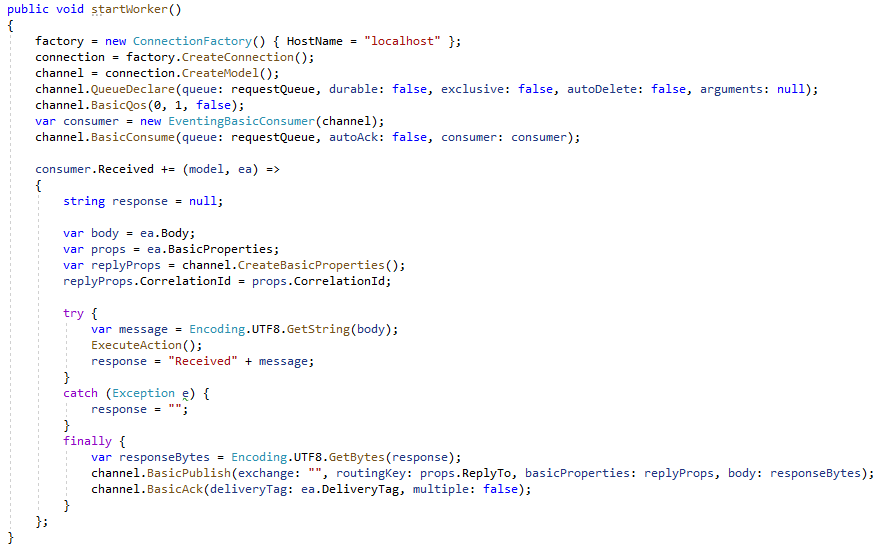
\includegraphics[scale=0.6]{RPCWorkerWhite.png}
	\caption[Screenshot]{RPC-Empfänger}
\end{figure}

In Abbildung 2.5 sehen wir ein Beispiel für einen Empfänger. Als erstes wird eine Verbindung zum Server aufgebaut und die Anfrage-Queue deklariert. Zusätzlich konfigurieren wir den Server nur eine unbestätigte Nachricht pro Queue zu erlauben. Wird dieser Wert erreicht, so werden keine Nachrichten mehr von der Queue verteilt. Dann wird ein Konsument erzeugt und dem Event Received via Lambda-Ausdruck eine Funktion übergeben, die auf empfangene Nachrichten reagiert. Innerhalb dieser wird die Nachricht ausgelesen und mit dem ausgelesenen Informationen eine Methode aufgerufen. Daraufhin schickt sie die Rückgabe der Methode an die Antwort-Queue. Zu guter Letzt wird der Konsument dann auch an die Anfrage-Queue angehängt.

Den Sender, oder auch RPC-Client genannt, implementierte ich an der Stelle, an welcher auch normalerweise der HTTP-Aufruf für eben diese Funktion stattfand.

\begin{figure}[h!]
	\centering
	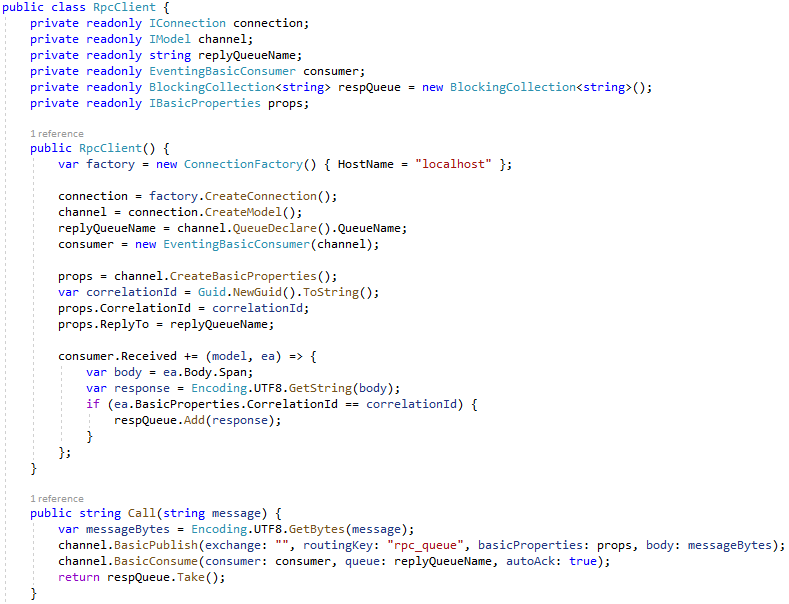
\includegraphics[scale=0.7]{RPCKlientWhite.png}
	\caption[Screenshot]{RPC-Sender}
\end{figure}

Abbildung 2.6 zeigt einen Beispiel-Sender. Er baut wie schon der Empfänger zuerst eine Verbindung zum Server auf. Danach erzeugt er Eigenschaften für die Nachricht und befüllt diese mit einem zuvor erzeugten Namen für die Antwort-Queue und einer zufälligen correlation\_id. Nun wird nur noch dem Konsument eine Funktion übergeben, die den Inhalt der Nachricht als Zeichenkette zwischenspeichert. Wenn nun die Call-Methode aufgerufen wird, wird eine Nachricht and die Anfrage-Queue gesendet und direkt danach der Konsument an die Antwort-Queue angehängt. Wurde die Antwort empfangen wird nun die zwischengespeicherte Zeichenkette zurückgegeben und aus dem Zwischenspeicher entfernt.

Nachdem ich also eine Methode hatte Zeichenketten mit dem Message Broker austauschen zu können, musste ich nun entscheiden wie ich die Übergabeobjekte in solch eine Zeichenkette umwandeln sollte, so dass diese auch am Empfänger zurückübersetzt werden konnten.
Ich entschied mich dafür die Objekte in eine JSON-Zeichenkette umzuwandeln, da dies das Rückübersetzen in ein Objekt sehr einfach gestaltete und ich bis zu diesem Zeitpunkt aus den vorherigen Aufgaben schon mehrere Erfahrungen zum Umgang mit JSON-Objekten hatte. 
Da es sich aber um komplexe Objekte handelte, die nicht nur Basisdatentypen als Werte hatten, musste ich den Übersetzer der JSON-Bibliothek, die ich verwendete, anpassen, so dass innere Objekte der Anfrage mit übersetzt werden konnten. 
Dann machte ich mich langsam daran, gezielt überflüssigen Code zu entfernen, solange bis nur noch der Kern der Funktion über war.

Den Prototypen zum Fanout-Exchange implementierte ich als Dead-Letter-Exchange, eine Art Exchange, den man bei der Initialisierung einer Queue angeben kann. An ihn werden Nachrichten gesendet, wenn diese Nachrichten eine in der Queue gesetzten Time-To-Live (TTL) überschreiten.

\section{Containervirtualisierung mit Docker} \label{docker}
Docker ist ein Werkzeug zur Erstellung und Verwaltung von Containern. 
Container sind kleine voneinander unabhängige Umgebungen in denen Programme lauffähig und von außerhalb gezielt erreichbar sind. Sie werden dafür eingesetzt eine Anwendung von äußeren Einflüssen zu befreien. Ihre Prämisse lautet, wenn eine Anwendung auf einem System funktioniert, funktioniert sie auf allen Systemen. Ein Container hat für gewöhnlich nur das nötigste installiert um lauffähig zu sein, alles andere wird vom Entwickler selbst beigesteuert. Was ihnen wiederum einen entscheidenden Vorteil im Vergleich zu einer virtuellen Maschine (VM) gibt. Aber nicht nur das. Einen Container aufzusetzen ist auch mit um einiges weniger Aufwand verbunden als das Aufsetzen einer VM. 

\subsection{Grundlagen der Containervirtualisierung}

Auch wenn Containervirtualisierung eine Art der Virtualisierung ist, laufen hierbei die Container nicht über ein Gastbetriebssystem, sondern befinden sich trotzdem auf ihrem Hostbetriebsystem. Auch wenn sie strikt getrennte Programminstanzen mit allesamt eigenen Abhängigkeiten und Ressourcen sind, teilen sie sich den selben Systemkernel. 

\begin{figure}[h!]
\centering
	\begin{subfigure}{0.4\linewidth}
		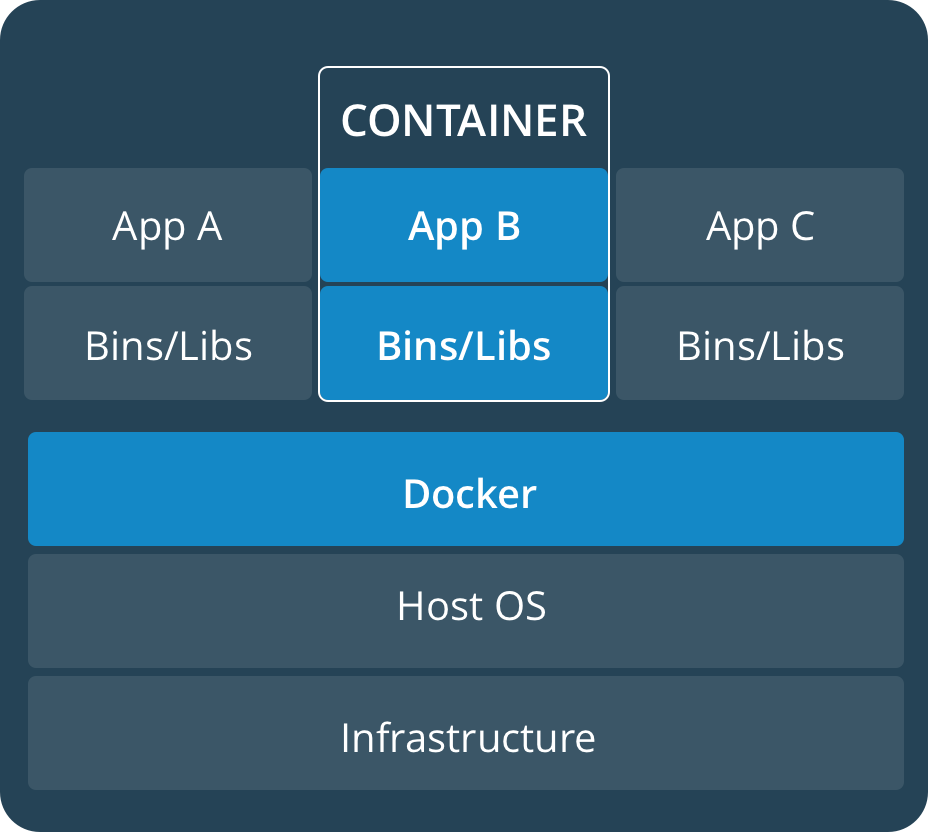
\includegraphics[scale=0.2]{DockerContainer.png} 
	\end{subfigure}
	\hspace*{1 cm}
	\begin{subfigure}{0.4\linewidth}
    	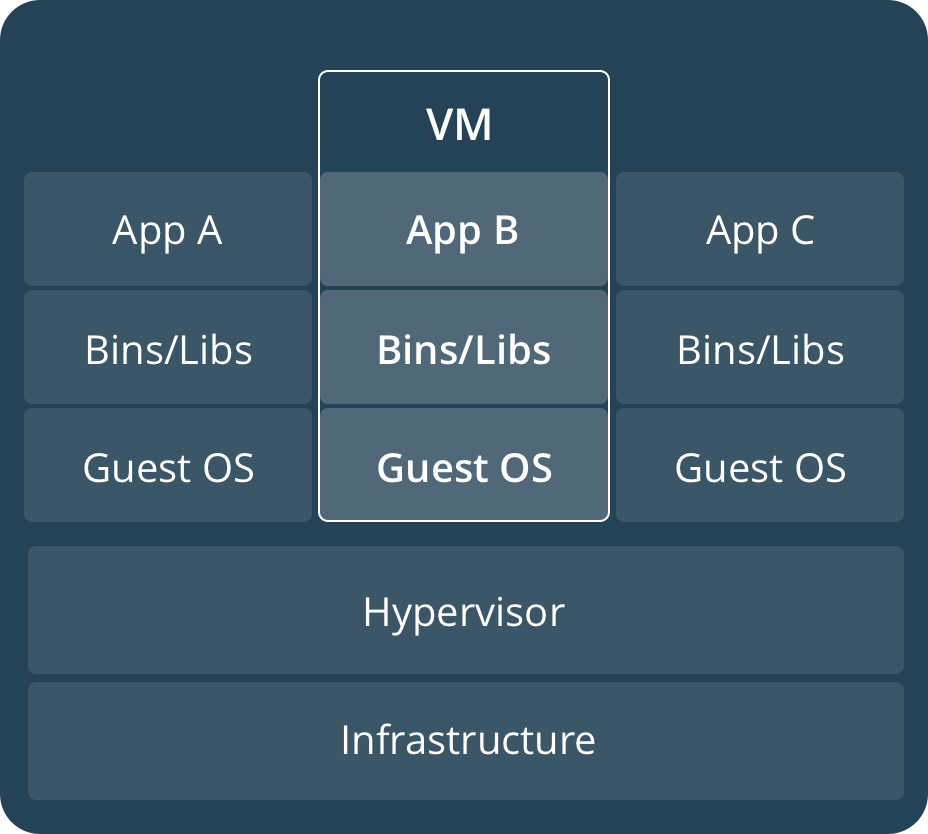
\includegraphics[scale=0.2]{DockerVM.png}
	\end{subfigure}
	\caption[https://docs.docker.com/get-started/]{Containervirtualisierung im Vergleich zu klassischer Virtualisierung.}
\end{figure}

Auf Abbildung 3.1 sehen wir die Containervirtualisierung im Vergleich zur klassischen Virtualisierung. Es ist leicht zu erkennen, dass durch die Einsparung des Gastbetriebssystems auf jeder Instanz wertvoller Speicherplatz erhalten werden kann. 

Dieser Vorteil wird aber erst bei einer größeren Anzahl an Instanzen richtig ersichtlich, weswegen diese Art der Virtualisierung bei verteilten Systemen zum Einsatz kommt. Ein verteiltes System ist ein System in dem die einzelnen verschiedenen Funktionen, die das System erfüllt, von unabhängigen, getrennten Komponenten erfüllt werden, die auf eine dynamische Weise miteinander verbunden sind. So wird es ein Einfaches dieses System horizontal zu Skalieren. Das Heißt, Instanzen des zu Skalierenden hinzuzufügen. Durch die dynamische Einbindung aller Komponenten wird sicher gestellt, dass die Last nun auf alle Instanzen des selben Typs gleichmäßig verteilt sind. Dies geschieht zum Beispiel mit einem Load Balancer. Mit einem Message Broker ist ähnliches zu erreichen.

\subsection{Docker Grundlagen}

Docker ist nun eine Plattform auf der wir mit Containern interagieren können. Das heißt unter anderem Container erzeugen und löschen, Ports teilen und Speicher zuteilen. Ein Container wird mit einem Image erzeugt. Ein Image ist ein Abbild der auszuführenden Programminstanz und wird aus einer Registry, einer zentralen Sammelstelle für Images, gezogen. Docker Images werden mit Dockerfiles erzeugt und können dann lokal verwaltet und auf externe Registries geschoben werden. Da mehrere Instanzen des selben Containers auch mehrere Anwendungen auf dem selben Port und der selben Adresse heißen würde, muss man auf die Ports, die von der Anwendung verwendet werden, von anderen Ports verweisen. Dies nennt sich Port-Mapping. 
Docker bietet auch Container mit Netzwerken zu verbinden, so dass ein DNS Containernamen auf ihre IP-Adressen übersetzt. Es gibt zwar auch Standardlösungen für diese Netzwerke, auf denen aber die Auflösung von Containernamen aber nicht möglich ist. Deshalb ist es ratsam diese Netzwerke selbst zu definieren. Ein anderes Konzept, das Docker einführt, ist Volume. Ein Volume ist eine Art Speicher mit dem sich Container verbinden und es dann benutzen können.
Container können über die Kommandozeile mit dem Befehl  \emph{docker run example/image:test} gestartet werden. Dabei können zahlreiche Parameter mitgegeben werden. Mit \emph{-p} können so Port-Mappings erstellt werden. Die lokalen Images können mit \emph{docker images} eingesehen werden. Mit \emph{docker ps} werden die laufenden Container angezeigt. Möchten wir auch die beendeten Container aufgelistet haben, so fügen wir das Kürzel \emph{-a} an. Wenn ein Container gestoppt werden soll geht dies mit \emph{docker stop container\_id}, für das entfernen \emph{docker rm container\_id}. Images werden mit \emph{docker rmi image\_id} entfernt.  

\begin{figure}[h!]
	\centering
	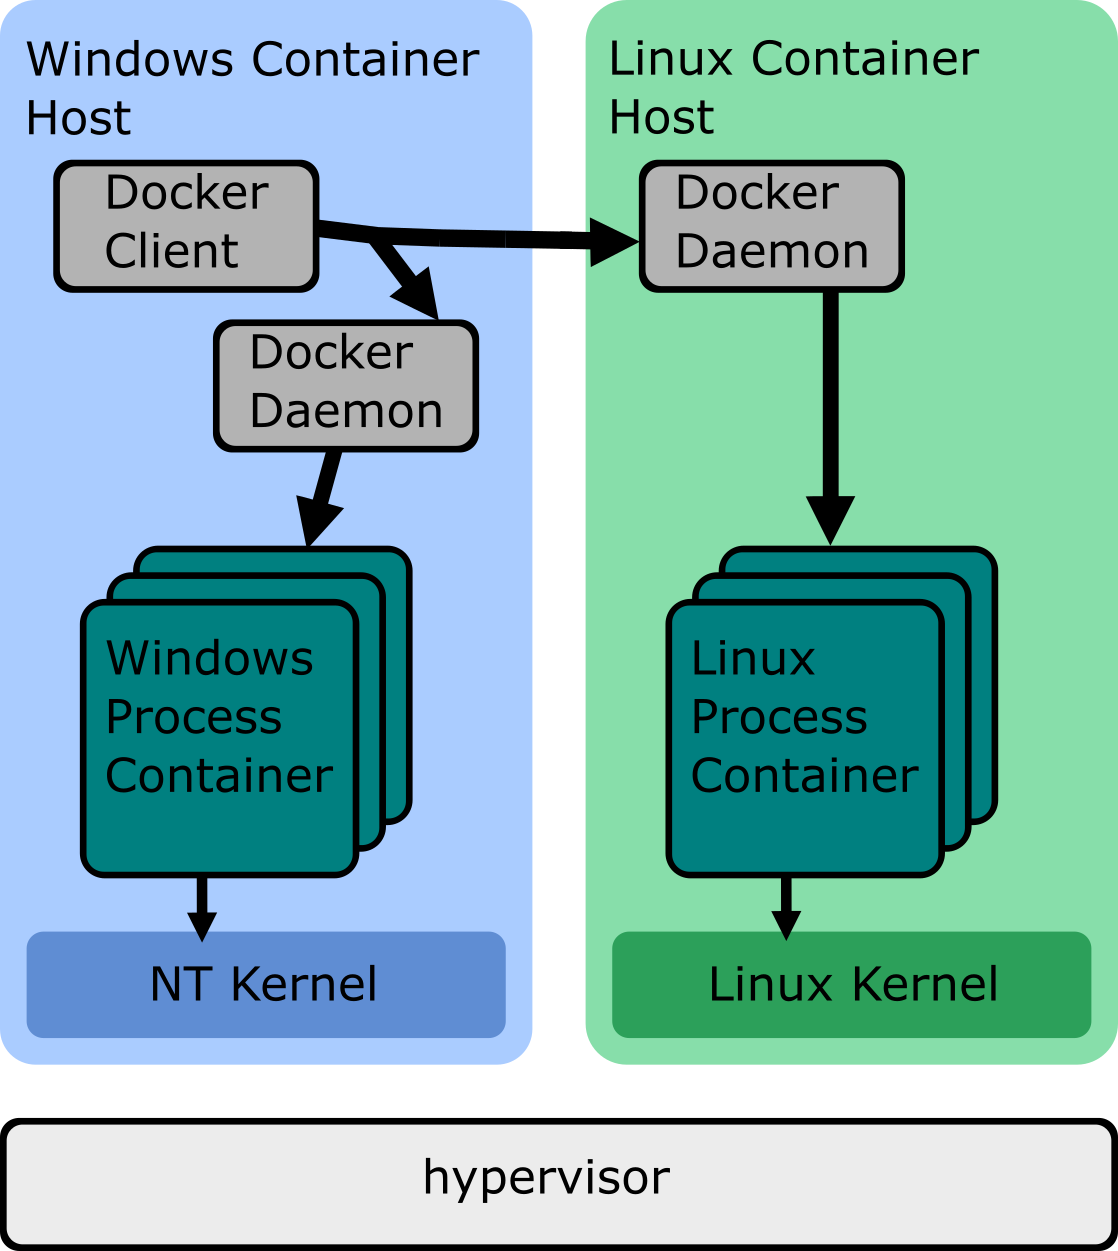
\includegraphics[scale=2]{DockerWindows.png}
	\caption[https://docs.microsoft.com/de-de/virtualization/windowscontainers/deploy-containers/linux-containers]{Linux Container auf Windows}
\end{figure}

Für gewöhnlich werden Linux-Container verwendet, auch unter Windows. Docker erstellt dafür dann eine VM, die das gewünschte Hostbetriebssystem so zur Verfügung stellt. Das wird auf Abb. 3.2 verdeutlicht. 

\subsubsection{Dockerfile}

Wie schon zuvor erwähnt wird mit einem Dockerfile ein Image unserer Anwendung erstellt. 

\begin{figure}[h!]
	\centering
	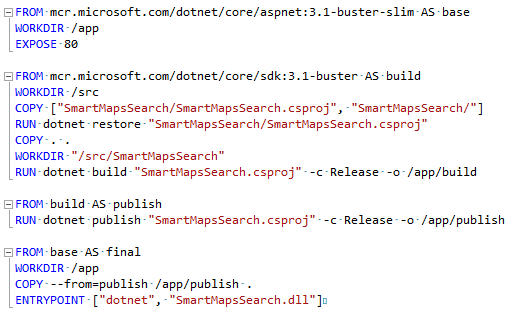
\includegraphics[scale=1]{DockerfileWhite.png}
	\caption[Screenshot]{Beispiel für einen Dockerfile}
\end{figure}

In Abb. 3.3 sehen wir wie ein Dockerfile exemplarisch aussehen könnte. Als erstes wird eine Basis referenziert die unser Image braucht um ausgeführt werden zu können. In diesem Fall ist dies .Net Core 3.1. Danach geben wir die Anweisung den Port 80 für diese Anwendung freizugeben. Nun wird alles Programm relevante in den Kontext gezogen, gebaut und veröffentlicht. Zuletzt wird ein Einstiegspunkt gesetzt, das heißt einen Befehl, der bei Start des Containers aufgerufen wird um die Anwendung auszuführen. 

Der \emph{FROM} Befehl, den wir mehrfach in dem Dokument finden können, initialisiert ein Basis Image und wird im weiteren dazu verwendet die verschiedenen Phasen während des Bauvorgangs zu trennen. In der vorletzten Zeile finden wir eine \emph{--from} Anweisung, die aussagt, dass hier auf den Kontext des Images \emph{publish}, das zuvor Initialisiert wurde, zugegriffen wird.

\begin{figure}[h!]
	\centering
	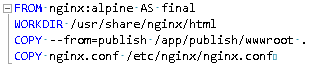
\includegraphics[scale=1]{DockerfileBlazor.png}
	\caption[Screenshot]{Webserver als Basisimage}
\end{figure}

Im Falle einer statischen Website, die von einem Blazor-WebAssembly-Projekt erzeugt wird, muss diese zwar mit .Net gebaut werden braucht aber keine Runtime-Umgebung, sonder benötigt einen Webserver.
Dies wird wie schon beschrieben erreicht indem wir die Basis wechseln und die gebauten Daten auf das neue Basisimage ziehen, wie auf Abb. 3.4 gezeigt. Ein Einsprungpunkt wird in diesem Fall nicht benötigt.

Um einen Dockerfile nun ausführen zu können und so ein Image zu erstellen müssen wir in der Kommandozeile den Befehl \emph{docker build .} in dem jeweiligen Ordner ausführen. Damit wir das Image später besser referenzieren können, lohnt es sich dem Image ein Tag, zu geben. Dies machen wir mit dem Kürzel \emph{-t}. Der Dockerfile kann mit dem Kürzel \emph{-f} angegeben werden. So kann auch auf eine andere Position in der Ordnerstruktur hingewiesen werden.

Images erzeugen zu können ist in Hinblick auf Kubernetes unerlässlich.

\subsubsection{Docker-Compose}

Mit Hilfe von Docker-Compose lassen sich Container vollständig konfiguriert und durch das Ausführen eines einzelnen Dokumentes starten. Das ermöglicht dem Nutzer komplexe Anwendungssysteme mit nur einem simplen Befehl ausführen zu können. 

\begin{figure}[h!]
	\centering
	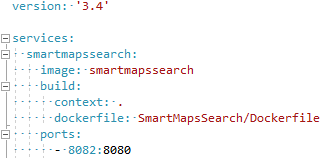
\includegraphics[scale=1]{DockerComposeMin.png}
	\caption[Screenshot]{Beispiel für Docker-Compose}
\end{figure}

Dabei ist Docker-Compose sehr simpel aufgebaut und wird mit der Auszeichnungssprache YAML spezifiziert. Im Beispiel, das in Abb. 3.5 zusehen ist, wird ein Container namens \emph{smartmapssearch} definiert, der ein gleichnamiges Image benutzt. Es werden weiterhin ein Port-Mapping hinzugefügt und Information zum Bauen des Images angegeben. Gebaut wird das Image wie zuvor mit einem Dockerfile, dessen Position und Namen wir angeben. 

Mit Docker-Compose können aber auch Volumes und Netzwerke hinzugefügt werden, die natürlich auch gleich an Container angebunden werden können.

\section{Skalierung mit Kubernetes} \label{kubernetes}
Kubernetes ist ein Werkzeug zur Erstellung und Verwaltung von Containerclustern. Containercluster sind Verbünde von einzelnen Containern die 

\subsection{Kubernetes Komponenten}

\subsection{Horizontale Skalierung}

\subsection{GitLab CI}

\subsection{Helm}

\subsection{Umsetzung}

\section{Stand des Projekts} \label{project_status}

\section{Fazit}\label{conclusion}
%Und jetzt spitzt das warme Blut aus dem Hals der letzten Sau. Und mit ihr stirbt ein kleines Stück Geschichte unserer Stadt. Der Sau ist es egal, doch wir wissen es genau. Der Bagger macht viel mehr als nur den alten Schlachthof platt. 

\newpage

%-----------------------------------------------------------------
% Ab hier => Literaturverzeichnis + temporäre Kommentare und Tests
%-----------------------------------------------------------------

\printbibliography
\addcontentsline{toc}{section}{Literaturverzeichnis}
\end{document}